% !TeX encoding   = UTF-8
\documentclass[12pt]{article}

\usepackage{sbc-template}

\usepackage{graphicx,url}
\usepackage[brazil]{babel}
\usepackage[utf8]{inputenc}
\usepackage{graphicx}	%Package para figuras
\usepackage{tabularx}
\usepackage{multirow} 
\usepackage[T1]{fontenc}
\usepackage{amsmath}
\usepackage{amsfonts}
\usepackage{amssymb}
\usepackage{makeidx}
\usepackage{graphicx}
\usepackage{lmodern}
\usepackage{epsfig}
\usepackage[linesnumbered,ruled,vlined]{algorithm2e}
%\usepackage[left=2cm,right=2cm,top=2cm,bottom=2cm]{geometry}

     
\sloppy

\title{Projeto e Análise de Algoritmos\\ Trabalho Prático 1 - Paradigmas}

\author{Vagner Clementino\inst{1}}

\address{Departamento de Ciência da Computação\\
	   Universidade Federal de Minas Gerais (UFMG)\\  
  \email{vagnercs@dcc.ufmg.br}
}

\begin{document} 

\maketitle

%\begin{abstract}
%  This meta-paper describes the style to be used in articles and short papers
%  for SBC conferences. For papers in English, you should add just an abstract
%  while for the papers in Portuguese, we also ask for an abstract in
%  Portuguese (``resumo''). In both cases, abstracts should not have more than
%  10 lines and must be in the first page of the paper.
%\end{abstract}
     
\begin{resumo} 
 TO DO
\end{resumo}


\section{Introdução}
\label{sec:intro}

Apesar da crença um cérebro maior não indica maior inteligência. Um contraexemplo bastante conhecido é Albert Einsten, cujo volume de seu cérebro não era maior do que o da média. Com a melhoria das imagens de ressonância magnética (IRM), diversos estudos vêm sendo proposto com o objetivo de correlacionar o \textit{volume} do cérebro com o \textit{Quociente de Inteligência} (QI). Um estudo utilizando imagens concluiu que a correlação entre QI e o volume do cérebro é consistente, todavia, as correlações fracas, e não há como comprovar uma relação direta. Em síntese: ser um \textit{``cabeção"} não é indicativo de inteligência.

A fim de refutar de vez esta crença, este trabalho se propõem em analisar os dados de \emph{peso} e \emph{QI} de um determinada população, com o objetivo de encontrar o maior número de pessoas cujo o peso do seu cérebro é menor, contudo, com um QI maior. O problema será formalmente definido na Seção \ref{sec:definicao}{}.

Este documento está estruturado como segue. A Seção \ref{sec:definicao} define formalmente o problema, fazendo uma relação do mesmo com o problema da \textit{Longest increasing subsequence}{}; a Seção \ref{sec:solucoes} apresenta as três soluções propostas para resolver o problema: \textsc{Força Bruta} (subseção \ref{subsec:forca_bruta}{}), \textsc{Gulosa} (subseção \ref{subsec:guloso}) e \textsc{Programação Dinâmica} (subseção \ref{subsec:pd}); a Seção \ref{sec:experimentos}{} faz uma discussão sobre resultados os experimentais de cada solução; a Seção \ref{sec:conclusao} discorre sobre as conclusões do trabalho.

\section{Definição Formal do Problema}
\label{sec:definicao}

O problema pode ser definido formalmente da seguinte forma. Dados $C=\langle c_1, c_2, \ldots, c_n\rangle$ um conjunto de indivíduos de tamanho $n$, bem como $P=\langle p_1, p_2, \ldots, p_n\rangle$ e $Q=\langle q_1, q_2, \ldots, q_n\rangle$, onde $p_i$ e $q_i$ representa, respectivamente, o peso e o QI do i-ésimo indivíduo. O problema consiste em encontrar o subconjunto $S \subseteq C$ tal que para todo $s_i,s_j\in S $ onde $ i < j$ $ p_i < p_j$  \textbf{e} $q_i > q_j$. Além disso, $|S|$ deve ser \textit{máximo}.

O problema proposto neste trabalho pode ser facilmente mapeado para um bem conhecido problema de otimização denominado \textit{Longest Increasing Subsequence - LIS}{}\cite{knuth2013art}{}. Para tanto, basta ordenar um dos conjuntos $P$ ou $Q$ de forma crescente ou decrescente. Por exemplo, caso o conjunto $P$ de forma decrescente, o problema se transforma em encontrar a maior \textit{LIS} no novo conjunto $Q^{'}$ que foi gerado pela ordenação de $P$.\footnote{Considera-se que para toda posição i em $P$ e $Q$ represente os dados do mesmo indivíduo}

O LIS é um problema bastante estudado e existem diversas abordagens na literatura para resolvê-lo. Este trabalho utilizou algumas destas referências nas soluções propostas na Seção \ref{sec:solucoes}{}.

\section{Soluções propostas}
\label{sec:solucoes}

Neste trabalho foi proposto três soluções para o problema utilizando os paradigmas \textsc{Força Bruta},  \textsc{Gulosa} e \textsc{Programação Dinâmica}{}. Para cada paradigma discute-se como foi realizada a modelagem, o funcionamento do algoritmo proposto e a análise da complexidade de tempo e de espaço. A descrição dos algoritmos será feita em mais alto nível por meio de pseudocódigo.

\subsection{Força Bruta}
\label{subsec:forca_bruta}

\subsubsection{Modelagem}
\label{subsubsec:model_fb}
O paradigma de Força Bruta é o único que garantidamente encontra uma solução ótima para qualquer problema computável. Contudo, o preço que se paga por esta aplicabilidade universal é o alto custo de tempo e/ou espaço necessário. A principal característica de uma abordagem Força Bruta é que ela faz uma \textit{busca integral no espaço de soluções} \cite{Kleinberg:2005:AD:1051910}{}. Neste sentido, ao desenvolvermos um algoritmo força bruta, ele deverá listar todas as possíveis soluções do problema para posteriormente definir a melhor entre as soluções válidas.

No contexto do problema estudado, o espaço de soluções consiste de todas as permutações dos elementos do \textit{power set} de $C$, cuja a notação é dada por $2^{C}$. Desta forma, o algoritmo a ser proposto deverá ser capaz de criar cada permutação possível de tamanho $1,2,\ldots, n$. Para cada permutação/solução criada deverá ser verificado se a solução é válida a fim de encontrar a melhor entre as válidas. Na próxima subseção descreveremos o algoritmo proposto.

\subsubsection{O Algoritmo Força Bruta}
\label{subsubsec:alg_fb}

O algoritmo \ref{algo:brute_force} apresenta em alto nível a abordagem Força Bruta utilizada. Por meio do método \textsc{GENERATE-ALL-SOLUTIONS} todas as possível soluções são geradas. A partir delas a solução ótima (de maior tamanho) é encontrada e posteriormente retornada $S_{best}$. O método \textsc{IS-VALID} verifica se uma da solução é valida verificando se cada par de item respeita as restrições do problema.

\begin{algorithm}
\SetKwFunction{ISVALID}{IS-VALID}
\SetKwFunction{GENERATEALLSOLUTIONS}{GENERATE-ALL-SOLUTIONS}
\DontPrintSemicolon % Some LaTeX compilers require you to use \dontprintsemicolon instead
\KwIn{As sequências finitas $C=\langle c_1, c_2, \ldots, c_n\rangle$, $P=\langle p_1, p_2, \ldots, p_n\rangle$ e $Q=\langle q_1, q_2, \dots, q_n\rangle$}
\KwOut{Uma sequência $S_{best} \subseteq C$ tal que atende as restrições do problema e seja máxima}

$U \gets $ \GENERATEALLSOLUTIONS{$C$}\;
$max \gets 0$\;
$S_{best} \gets \emptyset$\;
\For{\textbf{each} $S$ \textbf{in} $U$} {
   \If{\ISVALID{$S$}}{
   		\If{$S.legth() > max$}{
   		     $max \gets S.legth()$\;
   		     $S_{best} \gets S$\;
   		
   		}
   
   }
}
\Return{$S_{best}$}\;
\caption{{\sc BRUTE-FORCE} encontra a solução ótima listando todas elas.}
\label{algo:brute_force}
\end{algorithm}

\subsubsection{Análise de Complexidade}
\label{subsubsec:fb_analise_complexidade}

Conforme exposto anteriormente, na abordagem de Força Bruta é realizada uma busca em cada item do espaço de soluções do problema. Na subseção \ref{subsubsec:model_fb} discutiu-se que este espaço de solução $O(2^{n})$. Neste contexto, o método responsável por varrer o espaço de soluções necessariamente terá sua complexidade igual $O(2^{n})$. No algoritmo \ref{algo:brute_force} este trabalho é realizado pelo método \textsc{GENERATE-ALL-SOLUTIONS}{}. Como não as demais funções do algoritmo possuem complexidade inferiores, podemos concluir que o algoritmo de força bruta proposto possui ondem de complexidade de tempo igual a $O(2^{n})$.

No tocante a complexidade de espaço, o algoritmo necessita carregar os conjuntos $C$, $P$ e $Q$ a fim de poder gerar todas as soluções e verificar se elas são válidas. Apesar de no pior caso existir $O(2^{n})$ possíveis soluções, o sistema apenas armazena a melhor solução encontrada no momento. Partindo desta estratégia teremos um cutso de espaço igual a $O(1)$. Neste sentido, o algoritmo têm uma complexidade de espaço igual a $O(n)${}.

\subsection{Uma abordagem Gulosa}
\label{subsec:guloso}

Apesar do algoritmo de força bruta resolver o problema, conforme poderá ser observado na Seção \ref{sec:experimentos} onde descreve a análise experimental dos algoritmos, tal abordagem torna-se impraticável quando o tamanho da entrada cresce. Com o objetivo de encontrar uma solução de melhor desempenho, esta seção descreve uma solução baseada no paradigma \textit{Guloso}.

\subsubsection{Modelagem}
\label{subsubsec:model_guloso}
Um problema é passível de ser resolvido utilizando a abordagem Gulosa caso ele possua a propriedade da \texit{subestrutura ótima}{}. Um problema é dito ter subestrutura ótima se uma solução ótima pode ser construído de forma eficiente a partir de soluções ótimas de seus subproblemas \cite{Cormen:2009:IAT:1614191}{}. Vamos provar que o problema em  questão possui subestrutura ótima.

Iniciemos, sem perda de generalidade, ordenando o conjunto de entrada $C$ de forma descrescente pelo seu conjunto de pesos $P$. Conforme exposto na Seção \ref{sec:definicao} ao realizarmos a ordenação da entrada conforme proposto, o problema transforma-se em encontrar uma \texit{LIS} no novo conjunto de QI's $Q^{'}$ gerado.

Seja $S_{ij}$ a maior LIS entre os elementos $i$ e $j$ do conjunto  $Q^{'}$, conforme descrito no parágrafo anterior, tal que $1 \leq i \leq (n-1)$ e $i < j$. Desta forma, $S_{1n}$ é a solução ótima para o problema. Suponha que escolhamos um valor $k$ qualquer de modo que $ i \leq k < j$. As soluções $S_{ik}$ e $S_{(K+1)j}$ \texit{são ótimas} o que pode ser provado por absurdo. Suponha sem perda de generalidade que exita uma solução $S'_{ik}$ tal $|S'_{ik}| > |S_{ik}|$, a existência de $S'_{ik}$ vai contra a suposição de que $S_{ij}$ seja ótima.

Após provado que o problema apresenta subestrutura ótima já é possível propor um algoritmo guloso para o problema. A solução proposta é detalhada na subseção \ref{subsubsec:alg_guloso}.

\subsubsection{O Algoritmo Guloso}
\label{subsubsec:alg_guloso}

\subsection{Programação Dinâmica}
\label{subsec:pd}


Figure and table captions should be centered if less than one line
(Figure~\ref{fig:exampleFig1}), otherwise justified and indented by 0.8cm on
both margins, as shown in Figure~\ref{fig:exampleFig2}. The caption font must
be Helvetica, 10 point, boldface, with 6 points of space before and after each
caption.

\begin{figure}[ht]
\centering
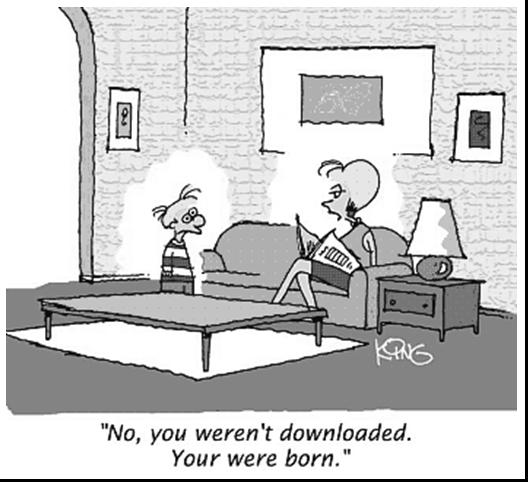
\includegraphics[width=.5\textwidth]{fig1.jpg}
\caption{A typical figure}
\label{fig:exampleFig1}
\end{figure}

\begin{figure}[ht]
\centering
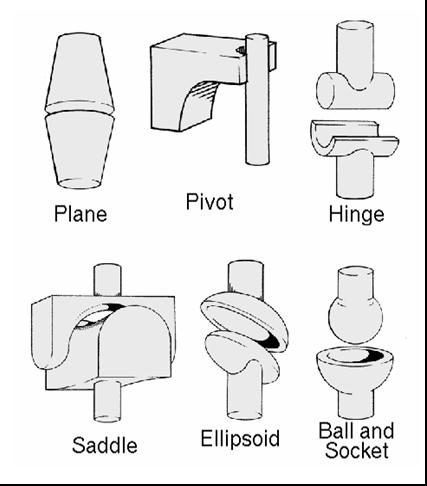
\includegraphics[width=.3\textwidth]{fig2.jpg}
\caption{This figure is an example of a figure caption taking more than one
  line and justified considering margins mentioned in Section~\ref{sec:figs}.}
\label{fig:exampleFig2}
\end{figure}

In tables, try to avoid the use of colored or shaded backgrounds, and avoid
thick, doubled, or unnecessary framing lines. When reporting empirical data,
do not use more decimal digits than warranted by their precision and
reproducibility. Table caption must be placed before the table (see Table 1)
and the font used must also be Helvetica, 10 point, boldface, with 6 points of
space before and after each caption.

\begin{table}[ht]
\centering
\caption{Variables to be considered on the evaluation of interaction
  techniques}
\label{tab:exTable1}
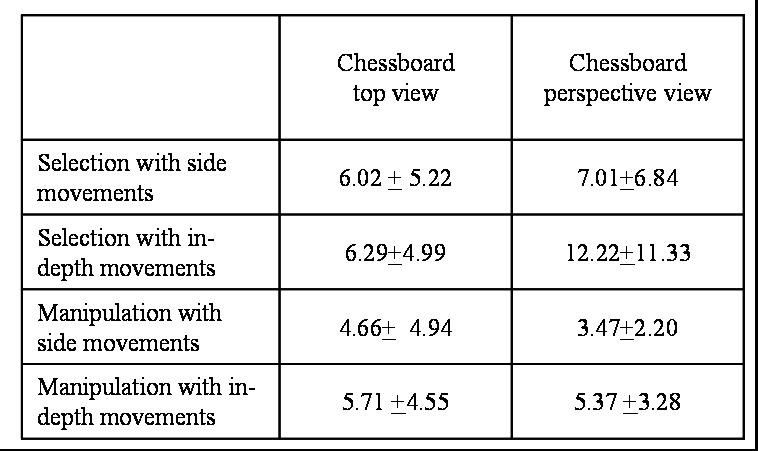
\includegraphics[width=.7\textwidth]{table.jpg}
\end{table}

\section{Análise Experimental}
\label{sec:experimentos}

All images and illustrations should be in black-and-white, or gray tones,
excepting for the papers that will be electronically available (on CD-ROMs,
internet, etc.). The image resolution on paper should be about 600 dpi for
black-and-white images, and 150-300 dpi for grayscale images.  Do not include
images with excessive resolution, as they may take hours to print, without any
visible difference in the result. 

\section{Conclusões}
\label{sec:conclusao}

Bibliographic references must be unambiguous and uniform.  We recommend giving
the author names references in brackets, e.g. \cite{knuth:84},
\cite{boulic:91}, and \cite{smith:99}.

The references must be listed using 12 point font size, with 6 points of space
before each reference. The first line of each reference should not be
indented, while the subsequent should be indented by 0.5 cm.

\bibliographystyle{sbc}
\bibliography{sbc-template}

\end{document}
